The given circle can be expressed as
\begin{align}
    \label{eq:chapters/11/11/1/7/given} 
    \norm{\vec{x}}^2  + 2\myvec{-2 & -4}\vec{x} - 45 = 0
\end{align}
where
\begin{align}	
	\vec{u} &= \myvec{-2\\-4},\, f = -45 \\
	\implies \vec{c} &= \myvec{2\\4},\,
	r = \sqrt{65}.	
\end{align}
See Fig. 
    \ref{fig:chapters/11/11/1/7/cicle}.
\begin{figure}[!htb]
    \centering
    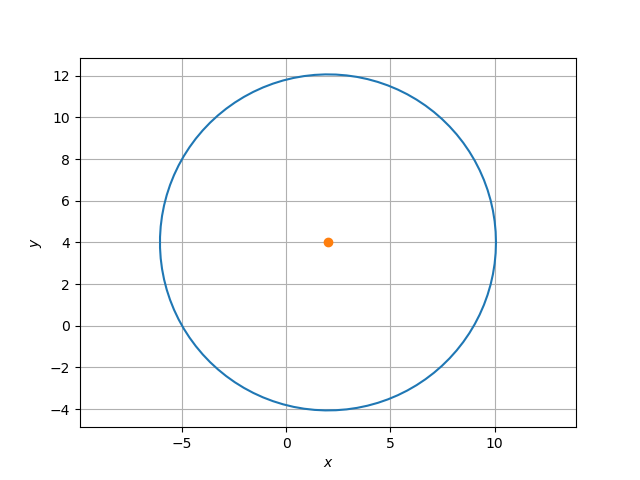
\includegraphics[width=\columnwidth]{chapters/11/11/1/7/figs/circle.png}
    \caption{}
    \label{fig:chapters/11/11/1/7/cicle}
\end{figure}

